\documentclass[pdf]
{beamer}
\mode<presentation>{}
%% preamble
\title{Discrete Element Method}
\author{Dinesh A}
\begin{document}

%% title frame
\begin{frame}
\titlepage
\end{frame}


%% normal frame
\begin{frame}{How to simulate?}

\begin{figure}[htbp]
\centerline{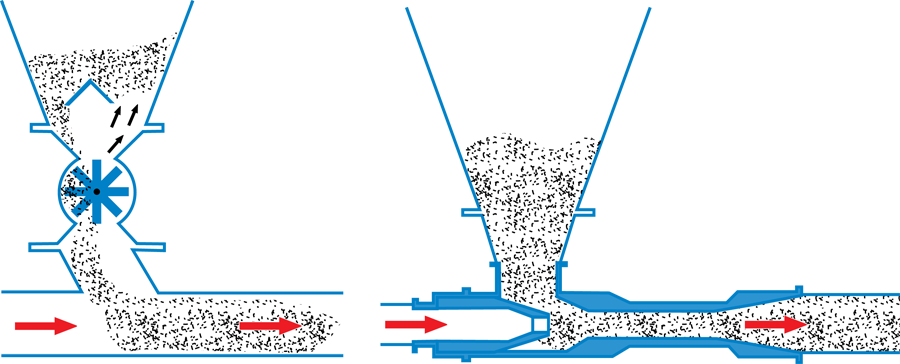
\includegraphics[]{hopper_real.png}}
\caption[]{Sand in a Hopper}
\end{figure}

\end{frame}


\begin{frame}{Or something like this}
\begin{figure}[htbp]
\centerline{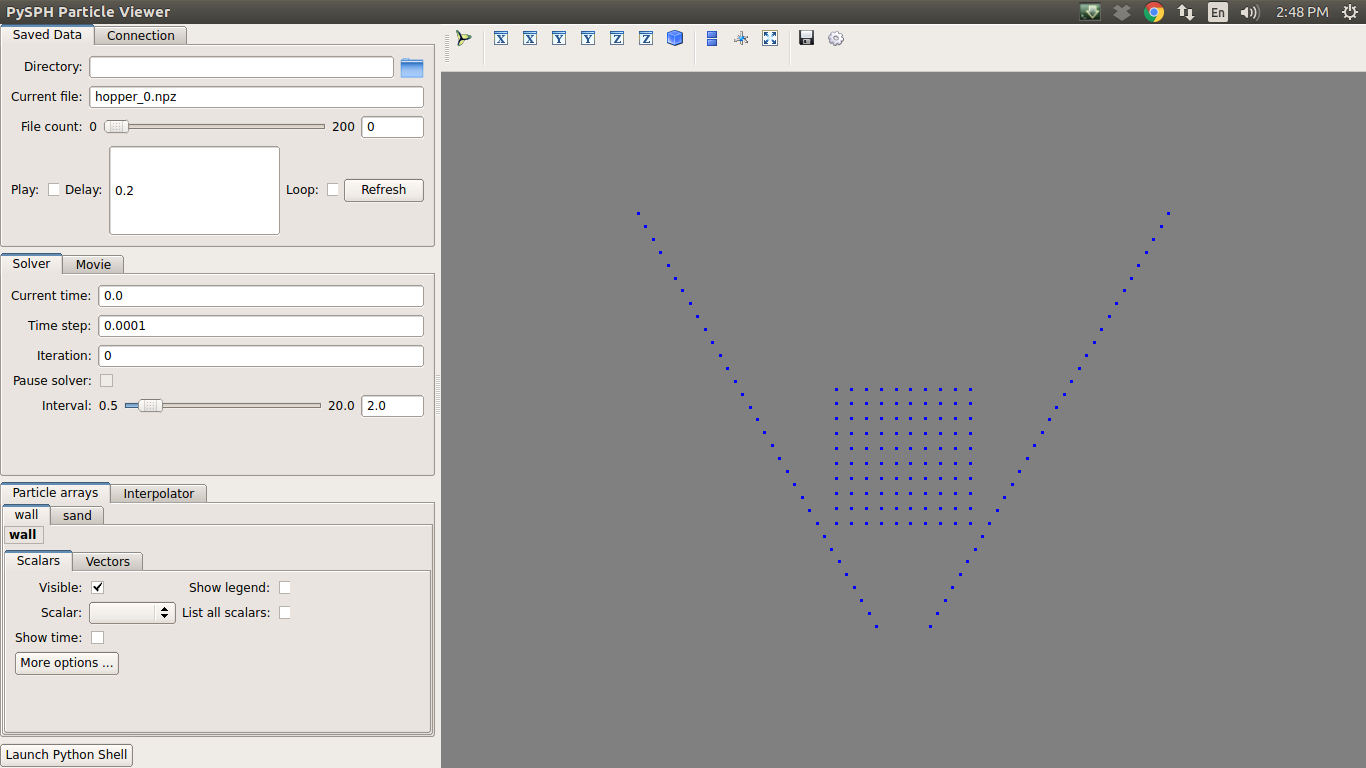
\includegraphics[width=10cm,height=10cm,keepaspectratio]{pysph_dem.png}}
\caption[]{\label{fig:pysph_dem} Hopper in PySPH}
\end{figure}

\end{frame}




\begin{frame}{Or something like this}


\begin{figure}[htbp]
\centerline{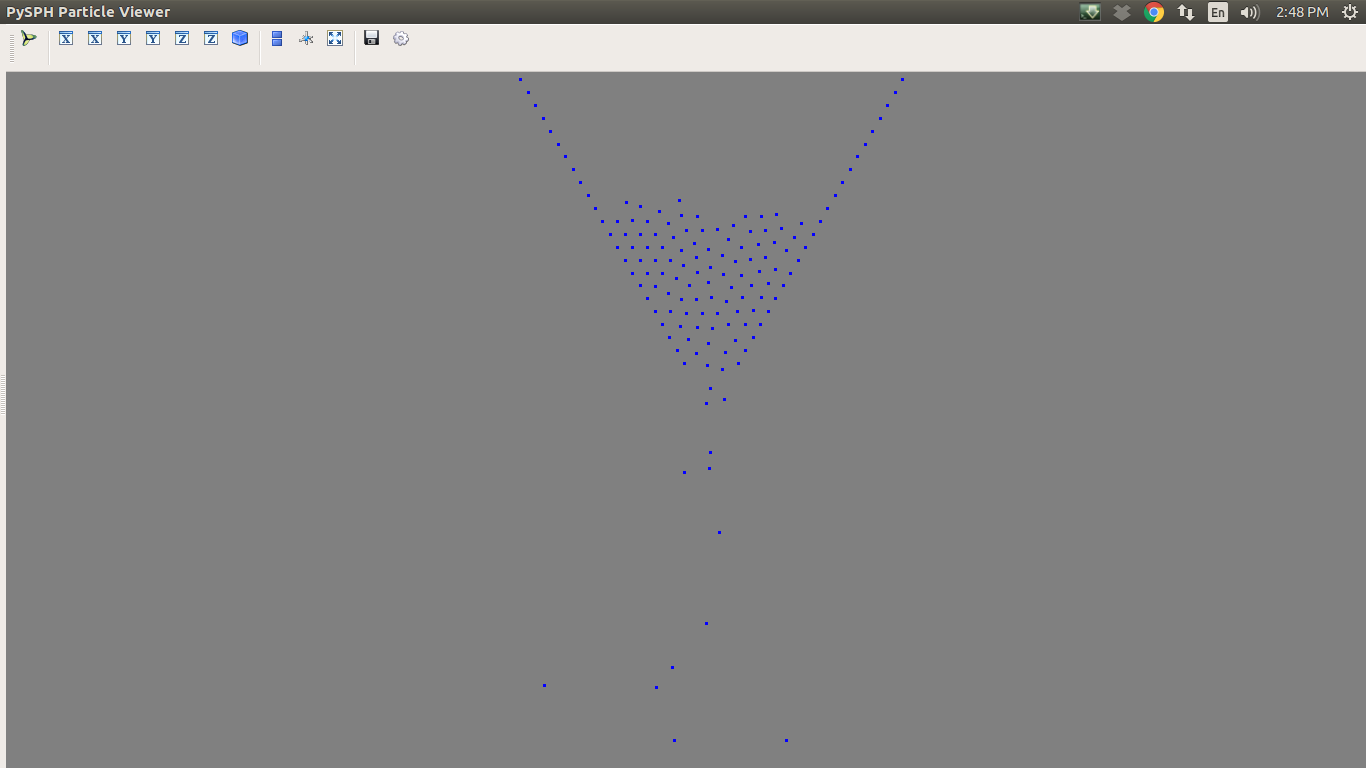
\includegraphics[width=10cm,height=10cm,keepaspectratio]{pysph_dem1.png}}
\caption[]{\label{fig:pysph_dem} Hopper in PySPH}
\end{figure}

\end{frame}














\begin{frame}{Use DEM}
  \frametitle{}


\begin{itemize}
\item Numerical method
\item Compute motion particles colliding
\end{itemize}

\end{frame}







\begin{frame}{Newtons second law}

\begin{align}
  \label{eq:newton_equation_of_motion}
  \frac{d^2 \vec{x}}{dt^2} = \vec{F}(\vec{x}, \vec{v}, m)\\
  \frac{d^2 \vec{\omega}}{dt^2} = \vec{M}(\vec{x}, \vec{v}, m)
\end{align}


\end{frame}





\begin{frame}{Define forces}

\begin{itemize}
\item Define forces
\item Say elastic
  \begin{itemize}
  \item Spring force
  \end{itemize}
\end{itemize}

\end{frame}




\begin{frame}{Spring Force}

  Apply only when they are in overlap

\begin{equation}
  \label{eq:overlap}
  \delta = (r_i + r_j) - |\vec{X}_{i} - \vec{X}_{j}|
\end{equation}


\begin{equation}
  \label{eq:normal_spring_force}
  \vec{F}_{nij}^S = -k_n \> \delta_n \> \vec{n}_{ij}
\end{equation}

Similarly for tangential direction

\begin{itemize}
\item Applicable when particle is rolling
\end{itemize}
\end{frame}



















\end{document}